\documentclass[sigconf, nonacm]{acmart}

\usepackage{amsmath,amsfonts}
\usepackage{graphicx}
\usepackage{textcomp}
\usepackage{multirow}
\usepackage{xcolor,colortbl}
\usepackage{algorithmic, algorithm}
\usepackage{caption}
\usepackage{subcaption}
\usepackage[draft]{fixme}
\usepackage{xspace}
\usepackage{hyperref} % makes cross-refs (biblio, figures, algos, ...) clickable

%% The following content must be adapted for the final version
% paper-specific
\newcommand\vldbdoi{XX.XX/XXX.XX}
\newcommand\vldbpages{XXX-XXX}
% issue-specific
\newcommand\vldbvolume{14}
\newcommand\vldbissue{1}
\newcommand\vldbyear{2020}
% should be fine as it is
\newcommand\vldbauthors{\authors}
\newcommand\vldbtitle{\shorttitle}
% leave empty if no availability url should be set
\newcommand\vldbavailabilityurl{}%http://vldb.org/pvldb/format_vol14.html}
% whether page numbers should be shown or not, use 'plain' for review versions, 'empty' for camera ready
\newcommand\vldbpagestyle{plain}

\newcommand{\tristan}[1]{\fxnote{\small \color{red} \textbf{From Tristan:}#1} \color{black}}
\newcommand{\timothee}[1]{\color{blue}\textbf{From Timothée:}#1\color{black}}
\newcommand{\mytodo}[1]{\color{red}\textbf{TODO:}#1\color{black}}
\newcommand{\keep}[0]{\textsc{keep}\xspace}

\begin{document}

\title{A heuristic to repartition large multi-dimensional arrays with reduced disk seeking}

\author{Timoth\'ee Gu\'edon$^{1,2}$, Val\'erie Hayot-Sasson$^1$, Tristan Glatard$^1$}

\affiliation{$^1$ Department of Computer Science and Software Engineering, Concordia University, Montreal, Canada\\
             $^2$ ESIEA school of engineering, France}

\begin{abstract}
Multi-dimensional arrays have become the main scientific data structures,
but their manipulation raises performance issues when they exceed memory
capacity. In particular, accessing specific array regions can require
millions to billions of disk seek operations, with important consequences
on I/O performance. While traditional approaches to address this problem
focus on file format optimizations, we are searching for algorithmic
solutions where applications control I/O to reduce
seeking. In this paper, we propose the \keep heuristic to minimize the
number of seeks required for the repartitioning of large multi-dimensional
arrays. The \keep heuristic uses a memory cache to reconstruct contiguous
data sections in memory. We evaluate it on arrays ranging from 85.7~GiB to
1~TiB, and with memory amounts ranging from 4 to 275~GiB. Repartitioning
time is reduced by a factor of up to 2.5, and seeking is reduced by four orders
of magnitude. Due to the effect of asynchronous writes to memory page cache
enabled by the Linux kernel, speed up is only observed for arrays that
exceed the size of working memory. The \keep heuristic could be applied in
platforms that manipulate large data arrays, as is commonly the case in
scientific imaging.
\end{abstract}

\listoffixmes

\newpage

\maketitle

%%% do not modify the following VLDB block %%
%%% VLDB block start %%%
\pagestyle{\vldbpagestyle}
\begingroup\small\noindent\raggedright\textbf{PVLDB Reference Format:}\\
\vldbauthors. \vldbtitle. PVLDB, \vldbvolume(\vldbissue): \vldbpages, \vldbyear.\\
%\href{https://doi.org/\vldbdoi}{doi:\vldbdoi}
\endgroup
\begingroup
\renewcommand\thefootnote{}\footnote{\noindent
This work is licensed under the Creative Commons BY-NC-ND 4.0 International License. Visit \url{https://creativecommons.org/licenses/by-nc-nd/4.0/} to view a copy of this license. For any use beyond those covered by this license, obtain permission by emailing \href{mailto:info@vldb.org}{info@vldb.org}. Copyright is held by the owner/author(s). Publication rights licensed to the VLDB Endowment. \\
\raggedright Proceedings of the VLDB Endowment, Vol. \vldbvolume, No. \vldbissue\ %
ISSN 2150-8097. \\
\href{https://doi.org/\vldbdoi}{doi:\vldbdoi} \\
}\addtocounter{footnote}{-1}\endgroup
%%% VLDB block end %%%

%%% do not modify the following VLDB block %%
%%% VLDB block start %%%
\ifdefempty{\vldbavailabilityurl}{}{
\vspace{.3cm}
\begingroup\small\noindent\raggedright\textbf{PVLDB Artifact Availability:}\\
The source code, data, and/or other artifacts have been made available at \url{\vldbavailabilityurl}.
\endgroup
}
%%% VLDB block end %%%


\vspace*{-0.3cm}
%----------------------------------------
\section{Introduction}
%----------------------------------------


% Multidimensional arrays are important
Multidimensional arrays are
used in many scientific disciplines as the main data structure~\cite{harris2020array}. In neuroimaging, our main application area, arrays
commonly store 2D, 3D or 3D+t brain images acquired from histology, magnetic
resonance imaging (MRI), or other modalities. Due to the improvement of
acquisition methods, it is now common for such images to exceed the amount
of working memory available on typical computers, requiring their
partitioning in blocks stored in independent files or in multiple HDF5
sections. BigBrain~\cite{Amunts1472}, for instance, is a human brain model
providing microscopic data at the resolution of 20 micrometres that comes
in the form of many 3D blocks. Partitioning large arrays enables efficient
queries, flexibility in adding new data~\cite{optimal_chuking}, granular data
transfers, and parallel processing with frameworks such as
Dask~\cite{matthew_rocklin-proc-scipy-2015}. Applications may adopt
different block geometries depending on their processing requirements, such
as 2D slices or 3D blocks.

% Seeks create performance issues
Manipulating large multidimensional arrays, however, come with performance
challenges related to the ordering and organization of array elements on
storage devices. In particular, reading or writing elements scattered in different
disk regions can generate millions to billions of \emph{seeks}, the
operations by which storage drives move to a different location, resulting
in important penalties on both SSD and HDD drives. Our goal is to minimize the number of seeks required when manipulating
large multi-dimensional arrays.

% Existing work
Currently, the main approach to this problem is to adapt the order of array
elements on storage devices to the type of queries done by applications.
For instance, the NDStore platform~\cite{lillaney2018building} orders voxels of 3D images
using Morton space-filling curves~\cite{morton1966computer}, so that nearby
voxels are stored at nearby disk addresses with high
probability. Other works determine from historical queries a
block shape that minimizes seeking
in future queries~\cite{optimal_chuking}.
While such approaches are efficient, they also require that data
be converted to a storage format specific to the application, which is
impractical and hampers data sharing. Instead, we are looking for
algorithmic approaches where applications control their I/Os to reduce seeking.

% Goal
This paper presents the \keep heuristic, an algorithm to reduce the
number of seeks created when repartitioning large multi-dimensional arrays in blocks of
arbitrary shape. Repartitioning may be triggered either by application requirements
 or for performance reasons, to improve
memory usage and I/O efficiency. For instance, the Python HDF5 library
\texttt{h5py} recommends a chunk size ``between 10~KiB and 1~MiB"~\cite{collette_2014}, while the Dask parallel processing framework
~\cite{matthew_rocklin-proc-scipy-2015} suggests a chunk size greater than
100~MB~\cite{rocklin_bourbeau_2019}.

The \keep heuristic leverages a memory cache to read and write data as
contiguously as possible, similarly to the "clustered" and "multiple"
algorithms described in~\cite{seqalgorithms}. The storage order of array
elements on disk is assumed to be known to the application, but unconstrained.
Implementations based on our algorithm could therefore use arbitrary file
formats. We focus on sequential algorithms, assuming that arrays are stored
on a single device and accessed by single-threaded I/Os. Extensions to parallel
environments are part of our future work. Although in practice seek times
depend on various factors, such as the distance between the initial and
target drive positions, we focus on minimizing seek \emph{numbers}, for
simplicity. Likewise, the effects of I/O optimizations such as page caching
or readahead will be discussed experimentally but not modelled.

In summary, the paper makes the following contributions:
\begin{itemize}
  \item We define the repartitioning problem for data arrays;
  \item We propose the \keep heuristic to the re-partitioning problem;
  \item We evaluate it for various memory amounts and data sizes.
\end{itemize}
The remainder of this paper presents these contributions and discusses the
validity and implications of our results.

% % need for tools to repartition
% Using chunked multidimensional arrays requires tools to efficiently split,
% merge, and ``resplit" or ``repartition" data files. Previous work in~\cite{seqalgorithms}
% showed that naive algorithms to split an array into several chunks or merge
% array chunks into one output file do not perform well due to millions of seeks
% occurring on disk. The present study is focused on sequential algorithms for
% repartitioning multidimensional arrays, letting the parallel and distributed
% cases as future work, although they are relevant, too. To the best of our
% knowledge, the repartition problem has not been extensively studied.

\begin{figure}
  \centering
  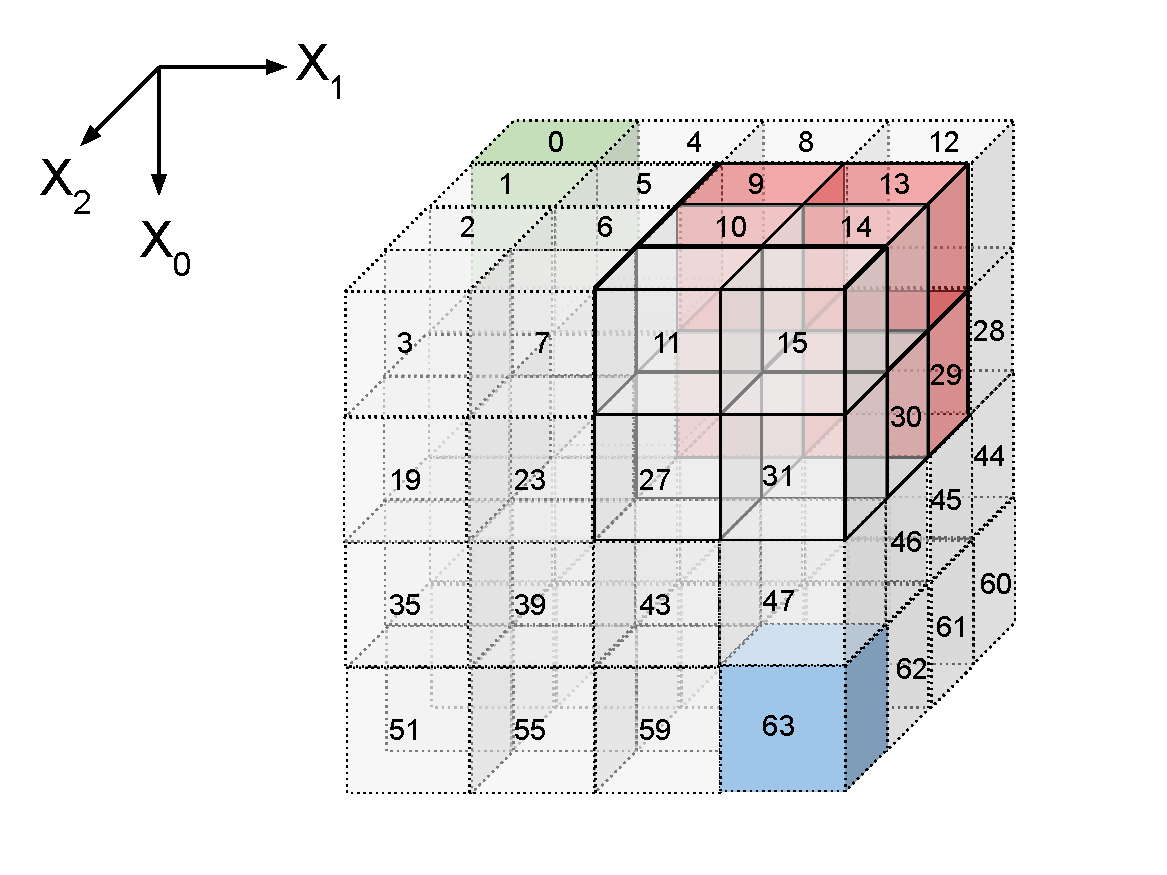
\includegraphics[width=0.5\textwidth]{./figures/figure_1.pdf}
  \caption{Ordering of 3D array elements in files in C order. The first stored element is colored in green,
  the last one is in blue. Seeking to the red elements is required when extracting the 3D block with plain borders.}
  \label{fig:seeks_and_rowmajor}
\end{figure}

\section{Problem definition and baseline}


For the sake of clarity and without loss of generality, we assume that
 files are written in row-major order (Fig.~\ref{fig:seeks_and_rowmajor},
 a.k.a. C order), where the fastest moving dimension in the file is the
 last dimension of the array, and the slowest moving dimension in the file
 is the first dimension of the array. This convention is, for instance, the
 one used in the HDF5 format ~\cite{hdf5}.

Accessing data from an array stored on disk generates seeks in two
situations: (1) when an array block is opened for reading or writing, and
(2) when the reading or writing process moves to a different address within
the block.

\subsection{The re-partitioning problem}

\begin{table}
  \caption{Notations}
  \begin{tabular}{ll}
    \multicolumn{2}{c}{\cellcolor{black!25}Mono-space fonts are used for array partitions}\\
    \texttt{A} & 3D array to repartition \\
    \texttt{inBlocks} & set of input blocks \\
    \texttt{outBlocks} & set of output blocks \\
    \texttt{readBlocks} & set of read blocks \\
    \texttt{writeBlocks} & set of write blocks \\

    &\\
    \multicolumn{2}{c}{\cellcolor{black!25}Square capitals are used for block shapes}\\
    A = ($A_0$, $A_1$, $A_2$) & shape of \texttt{A}\\
    I = ($I_0$, $I_1$, $I_2$)& shape of input blocks\\
    O = ($O_0$, $O_1$, $O_2$) & shape of output blocks\\
    R = ($R_0$, $R_1$, $R_2$) & shape of read blocks\\
    W = ($W_0$, $W_1$, $W_2$) & shape of write blocks\\
    &\\
    \multicolumn{2}{c}{\cellcolor{black!25}Round capitals are used for block end coordinates}\\

    $\mathcal{I}$ = ($\mathcal{I}_0$, $\mathcal{I}_1$, $\mathcal{I}_2$), \enskip $\mathcal{I}_d \subset \mathbb{N} $ & input block end coordinates \\
    $\mathcal{O}$ = ($\mathcal{O}_0$, $\mathcal{O}_1$, $\mathcal{O}_2$), \enskip $\mathcal{O}_d \subset \mathbb{N} $ & output block end coordinates\\
    $\mathcal{R}$ = ($\mathcal{R}_0$, $\mathcal{R}_1$, $\mathcal{R}_2$), \enskip $\mathcal{R}_d \subset \mathbb{N} $ & read block end coordinates\\
    $\mathcal{W}$ = ($\mathcal{W}_0$, $\mathcal{W}_1$, $\mathcal{W}_2$), \enskip $\mathcal{W}_d \subset \mathbb{N} $ & write block end coordinates\\
    &\\
    \multicolumn{2}{c}{\cellcolor{black!25}$n_X$ are used for block numbers}\\
    $n_I$ = number of input blocks\\
    $n_O$ = number of output blocks\\
    $n_R$ = number of read blocks\\
    $n_W$ = number of write blocks\\
  \end{tabular}
  \label{table:notations}
\end{table}

\begin{algorithm}[b]
  \caption{General re-partitioning algorithm}
  \label{algo:generalrepartition}
  \begin{algorithmic}[1]
    \STATE \textbf{Inputs}
    \STATE inBlocks: input blocks of shape $I$, stored on disk
    \STATE outBlocks: output blocks of shape $O$, to be written
    \STATE $m$: memory available
    \STATE
    \STATE \textbf{Outputs}
    \STATE none (outBlocks are written)
    \STATE
    \STATE \textbf{Algorithm}
    \STATE readBlocks, writeBlocks $\leftarrow$ getReadWriteBlocks($I$, $O$, $m$)
    \STATE initialize(cache)
    \FOR{readBlock in readBlocks}
      \STATE data $\leftarrow$ read(readBlock, inBlocks)
      \STATE \tristan{return complete blocks here, avoid for loop next}cache.insert(data)
      \FOR{writeBlock in writeBlocks}
        \IF{$\mathrm{readBlock} \cap \mathrm{writeBlock} \neq \emptyset$ \\
             \quad \textbf{and} cache.isComplete(writeBlock)}
          \STATE data $\leftarrow$ cache.pop(writeBlock)
          \STATE write(data, outBlocks)
        \ENDIF
      \ENDFOR
    \ENDFOR

  \end{algorithmic}
\end{algorithm}

We focus on 3D arrays for simplicity. Consider a 3D array \texttt{A} of shape $A =
(A_i, A_j, A_k)$, partitioned in uniformly-shaped input blocks of shape $I =
(I_i, I_j, I_k)$ stored on disk. Our goal is to re-partition the input
blocks into uniform output blocks of shape $O = (O_i, O_j, O_k)$,
where $O \neq I$. Notations are summarized in
Table~\ref{table:notations}.

We formalize the re-partitioning problem as in Algorithm~\ref{algo:generalrepartition}.
A re-partitioning algorithm takes a
list of input blocks \texttt{inBlocks}, a list of output
blocks \texttt{outBlocks}, and the amount of memory \texttt{m}
available for the algorithm. Subject to $m$, the algorithm determines (1)
\texttt{readBlocks}, a list of uniformly-shaped blocks of shape $R$ to be read from the
input blocks, and (2) \texttt{writeBlocks}, a list of blocks,
usually not uniformly-shaped, to be written to output blocks (line 10).
If read blocks and input blocks have a different shape, then reading read blocks requires
more than one seek. Similarly, if write blocks and output blocks have a different shape,
then writing write blocks requires more than one seeks. Input, output, read
and write blocks all form a partition of the 3D array \texttt{A}. The
main loop of the algorithm (line 12) loads one read block at a time (line
13), inserts it into a cache (line 14), and writes write blocks from the
cache when they are complete (lines 15 -- 20). Function \texttt{write} is assumed
to open each output block only once, and to write the required elements of \texttt{data} in it.

It should be noted that blocks are passed to the algorithm by reference,
not by data. Only variables \texttt{data} (lines 13, 17) and \texttt{cache}
(line 14) hold actual data, contributing to the consumed memory.

Since read and write blocks both represent a partition of $A$, all the
elements in \texttt{inBlocks} are read exactly once and written exactly once too. Other
problem formalizations may allow for input elements to be read and
discarded, to reduce seeking. Exploring such a trade-off
between seeks and redundant reads could be an interesting extension to this problem.

Our goal is to minimize the number of seeks done by the algorithm, which
occurs during reads (line 13) and writes (line 18). The re-partitioning
problem is therefore to find \texttt{readBlocks} and \texttt{writeBlocks} that
minimize the number of
seeks done by the algorithm, subject to the memory constraint $m$.

% Problem: re-partitioning of multi-dimensional arrays
% Find: readBlocks and writeBlocks
% Subject to: m
% Such that: seeks is minimal
% \tristan{formalize problem definition}.

Solutions of this problem materialize as implementations of function
\texttt{getReadWriteBlocks} (Alg.~\ref{algo:generalrepartition}, line 10). A
lower bound on the number of seeks for the repartitioning problem is $n_I +
n_O$, with $n_I$ the number of input blocks and $n_O$ the number of output
blocks. Indeed, input and output blocks all have to be opened at least
once, which requires a seek.

For simplicity, we require that all blocks in \texttt{readBlocks} have the
same shape $R$. We also equate the size of an array in memory as its
number of elements. To the best of our knowledge, no algorithm has been
proposed for the repartitioning problem.


\subsection{Baseline}

Our baseline algorithm for the repartitioning problem loads one input block
at a time ($R$=$I$), and directly writes it to the appropriate output
blocks ($W$=$R$). It assumes that input blocks fit in memory. The number of
generated seeks $s_b$
depends on how write blocks overlap with
output blocks in each dimension (Fig.~\ref{fig:baseline_figure}). To determine $s_b$, we define
$\mathcal{W}_d$ and $\mathcal{O}_d$, the sets of write and output block end
coordinates in dimension $d$:
\[
  \forall d \in \llbracket 1, 3 \rrbracket,
\]
\begin{equation}
  \mathcal{W}_d = \Big\{ iW_d, i \in \llbracket 1, A_d/W_d \rrbracket \Big\} \quad \mathrm{and} \quad
  \mathcal{O}_d = \Big\{ iO_d, i \in \llbracket 1, A_d/O_d \rrbracket \Big\} ~\label{eq:baseline-blocks}
\end{equation}
We then define the \emph{cuts} of the $i^{th}$ output block along dimension
$d$ as follows:
\[
  \forall i \in \llbracket 1, A_d/O_d \rrbracket,
\]
\[
  C_{i, d} = C_{i, d}\left(  \mathcal{W}_d, \mathcal{O}_d \right) = \Big\{ w \in \mathcal{W}_d, (i-1)O_d < w < iO_d \Big\}
\]
The number of output block pieces along dimension $d$ is then:
\[
  c_d = c_d\left(  \mathcal{W}_d, \mathcal{O}_d \right) =
               \sum_{i=1}^{A_d/O_d} \vert C_{i, d}\left(  \mathcal{W}_d, \mathcal{O}_d \right) \vert + 1 - \delta_{\vert C_{i, d}\left(  \mathcal{W}_d, \mathcal{O}_d \right) \vert, 0}
\]
where $\vert$ . $\vert$ is the cardinality operator and $\delta$ is the Kronecker delta \tristan{I dont think we need the 1 and delta}.
The number of \emph{matches} between block endings is:
\[
  m_d = m_d\left(  \mathcal{W}_d, \mathcal{O}_d \right) = \vert \mathcal{W}_d \cup  \mathcal{O}_d \vert  - c_d
  \]
Finally, the number of seeks created by the baseline algorithm is:
\begin{equation}
  s_b = A_0 A_1 c_2 +
      A_0 c_1 m_2 +
      c_0 m_1 m_2
       + n_I + (m_0+c_0)(m_1+c_1)(m_2+c_2) \label{eq:seeks-baseline}
\end{equation}
with $(m_0+c_0)(m_1+c_1)(m_2+c_2)$ the number of output block openings.

\begin{figure}
  \centering
  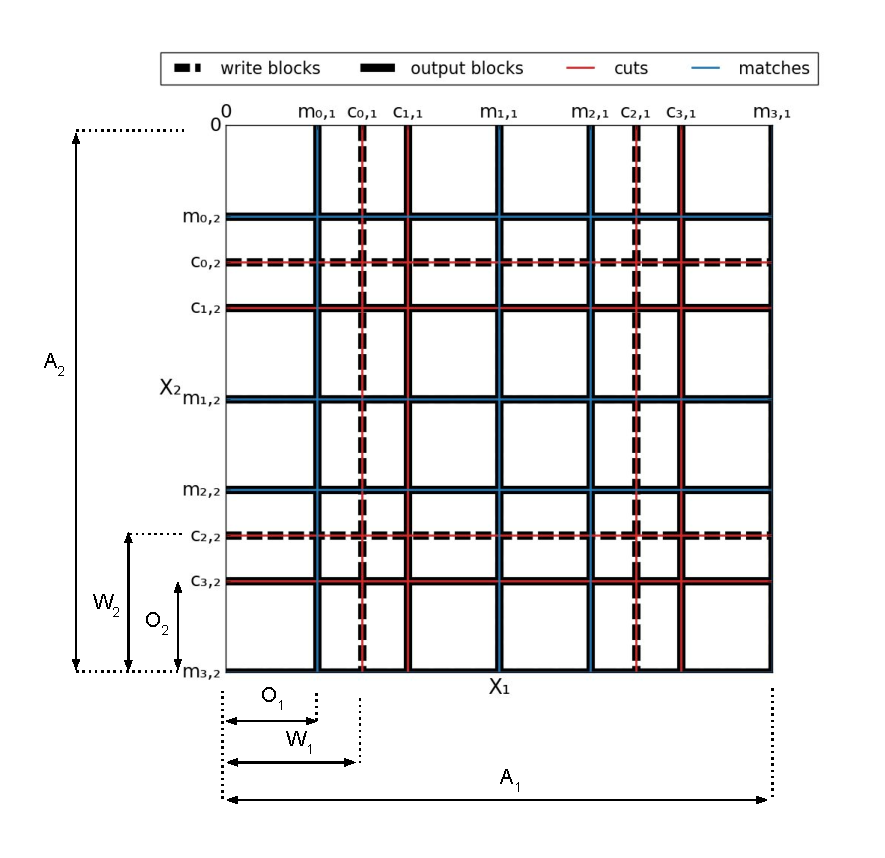
\includegraphics[width=0.5\textwidth]{./figures/baseline_figure.pdf}
  \caption{Overlapping of write and output blocks in the plan
  ($X_1$,$X_2$), showing cuts (red lines) and matches (green lines)}
  \label{fig:baseline_figure}
  \end{figure}

  As can be seen from Equation~\ref{eq:seeks-baseline}, cuts along dimension 2 generate $\mathcal{O}(A_0 A_1)$
seeks, which is prohibitive when \texttt{A} is large, cuts along dimension 1 generate $\mathcal{O}(A_0)$ seeks and cuts in
dimension 0 generate $\mathcal{O}(1)$ seeks. The \keep heuristic described
in the next section aims at avoiding cuts primarily in dimension 2, and if
possible in dimension 1 and 0. An experimental verification of the model will be provided in
Section ~\ref{sec:experiments}. \tristan{this is not a model, it is a count}

%----------------------------------------
\section{The \keep heuristic}
%----------------------------------------
As mentioned previously, the baseline strategy empties
the cache at each iteration, which generates many seeks when input and output
blocks have different shapes. Instead, the proposed
\keep heuristic keeps in cache the array elements that cannot be written
contiguously to the output blocks.

\subsection{Overview}

\begin{algorithm}
  \caption{\keep heuristic (implements \texttt{getReadWriteBlocks})}
  \label{algo:keep}
  \begin{algorithmic}[1]
    \STATE \textbf{Inputs}
    \STATE inBlocks: input blocks of shape $I$, stored on disk
    \STATE outBlocks: output blocks of shape $O$, to be written
    \STATE $m$: memory available
    \STATE
    \STATE \textbf{Outputs}
    \STATE readBlocks: a list of read blocks
    \STATE writeBlocks: a list of write blocks
    \STATE
    \STATE \textbf{Algorithm}
    \STATE readShapes = candidateReadShapes($I$, $O$, $A$)
    \STATE minSeeks = None
    \FOR{$R$ in readShapes}
      \STATE readBlocks = blocks($R$, $A$)
      \STATE writeBlocks = createWriteBlocks(readBlocks, outBlocks)
      \STATE mc = peakMemory($R$)
      \IF{mc > m}
      \STATE \textbf{continue} \COMMENT{Memory constraint cannot be fulfiled}
      \ENDIF
      \IF{$R$ == $\hat r$}
      \STATE bestReadBlocks = readBlocks
      \STATE \textbf{break} \COMMENT{$\hat r$ fulfills memory constraint}
      \ENDIF
      \STATE s = generatedSeeks($I$, $R$, writeBlocks, $O$)
      \IF{minSeeks == None or s < minSeeks}
      \STATE minSeeks, bestReadBlocks = s, readBlocks
      \ENDIF
    \ENDFOR
    \RETURN bestReadBlocks, writeBlocks
  \end{algorithmic}
\end{algorithm}
The \keep heuristic (Alg.~\ref{algo:keep}) is a brute-force search
of the best read shape among a list of candidates (line 11).
For each candidate read shape, it creates a list of write blocks (line
15), determines the memory consumed by this solution (line 16), and provided that the
memory constraint is respected, computes
the number of seeks created by the solution (line
24), and selects the read shape that minimizes the number of seeks (lines
25-27).

The \keep heuristic uses the following functions, described in the
remainder of this section: \texttt{candidateReadShapes} (line 11),
\texttt{blocks} (line 14), \texttt{createWriteBlocks} (line 15),
\texttt{peakMemory} (line 16), and
\texttt{generatedSeeks} (line 24).

\subsection{Candidate read shapes}

% Read shape candidates are generated as to avoid cuts along dimension 2
% during reads and writes. Ideally, the read shape would cover an exact
% number of input blocks, to avoid seeks during reads, and would include at
% least one output block, to avoid seeks during writes. In practice, this
% might not be possible due to memory limitations, since at each iteration
% the parts of the read block that are not written must remain in cache.

To generate candidate read shapes, we first define a shape $\hat r$ such
that in each dimension $d$, $\hat r_d$ is the smallest multiple of $I_d$
that is greater or equal to $O_d$:
\[
\forall d \in \{1, 2, 3\},
\]
\[
  \hat r_d = I_d \left \lceil \frac{O_d}{I_d} \right \rceil
%  \enskip \exists \hat k \in \mathbb{N}, \enskip \hat r_d = \hat kI_d \enskip \mathrm{and} \enskip \hat k I_d \geq O_d \enskip \mathrm{and} \enskip \forall k < \hat k, \enskip kI_d < O_d
\]

Using $\hat r$ as read shape minimizes seeking in the input blocks, as
in this situation each iteration reads input blocks completely, requiring a
single seek per input block. If there is enough memory to use write blocks
of shape $O$, then this solution also minimizes the seeks in the output
blocks, as output blocks can be written in a single seek too.

Function \texttt{candidateReadShape} returns the following shapes:
\[
  \Big\{ (C_0, C_1, \hat r_2) \in \mathbb{N}^3 \enskip / \enskip
          \forall i \in \{0, 1\}, \enskip \exists k_i \in \mathbb{N}, \enskip
           A_i = k_iC_i \enskip \mathrm{and} \enskip C_i \leq \hat r_i \Big\}
\]
The third coordinate of all read shapes is set to $\hat r_2$, to guarantee
that no cuts along dimension 2 will be made during reads. This assumes that
$m \geq \hat r_2$, i.e., a block of shape (1, 1, $\hat r_2$) fits in
memory, which seems reasonable. The other two coordinates are set to divisors of $A_0$ and $A_1$ which are
less than or equal to $\hat r_0$ and $\hat r_1$ respectively.

The candidate shapes are sorted first by decreasing $C_1$ values, then by
decreasing $C_0$ values. The first tested read shape is therefore
$\hat r$. While $\hat r$ is the optimal read shape, leading to a single
seek per input or output block, there is no obvious relation between the
other candidate shapes and the number of seeks that they generate since
this number depends on how input, read, write, and output blocks are
arranged. For this reason, the \keep heuristic returns if $\hat r$
respects the memory constraint (line 20-23), but it otherwise evaluates all
the other read shapes.

\subsection{Block order}

Creating uniform blocks from a block shape is
straightforward, but their order impacts the amount of data
stored in cache and therefore the peak memory consumption. For
simplicity, function \texttt{block} returns read blocks in the
order used for array elements on disk (C order in this paper).

\subsection{Creation of write blocks}

Function \texttt{createWriteBlocks} returns write blocks created from read and output blocks
as follows. For each read block,
eight write blocks are first created, defined as the $F_i$ blocks in
Figure~\ref{fig:nomenclature_overlaps}.
The $F_i$ blocks with $i \in [\![1;7]\!]$ are then merged
recursively with sub-blocks of neighboring read blocks, following the rules
in Table~\ref{tab:fusion}.
In fact, the $F_i, i \in [\![1;7]\!]$ are fused with $F_0$ blocks from
neighboring buffers.
The coordinates of $F_0$ are computed as follows: The upper-left coordinates are
$(0,0,0)$ in the referential of the read buffer, and the bottom-right coordinates
are defined to be the first output block's end coordinates encountered.

\begin{table}
  \centering
  \caption{Recursive merging of the initial write blocks. The first column
  identifies a sub-block of a read block (i.e., an initial write block),
  and the second column identifies the sub-block(s) of the neighboring read
  block(s) that are merged with the sub-block of the first column. For instance, sub-block $F_1$ is merged with sub-block $F_0$
  of the neighboring read block in dimension $X_2$. \tristan{target blocks are ORs}}
   \begin{tabular}{c|l}
   \rowcolor{black!25}
   Sub-block & Merged with \\
   \rowcolor{black!25}
             & (sub-block, neighbor direction) \\
   $F_0$     & -- \\
   \rowcolor{black!10}
   $F_1$     & ($F_0$, $X_2$) \\
   $F_2$     & ($F_0$, $X_1$) \\
   \rowcolor{black!10}
   $F_3$     & ($F_1$, $X_1$), ($F_2$, $X_2$) \\
   $F_4$     & ($F_0$, $X_0$) \\
   \rowcolor{black!10}
   $F_5$     & ($F_1$, $X_0$), ($F_4$, $X_2$)\\
   $F_6$     & ($F_2$, $X_0$), ($F_4$, $X_1$)\\
   \rowcolor{black!10}
   $F_7$     & ($F_3$, $X_0$), ($F_5$, $X_1$), ($F_6$, $X_2$)\\
   \end{tabular}
   \label{tab:fusion}
\end{table}

\begin{figure}
  \centering
  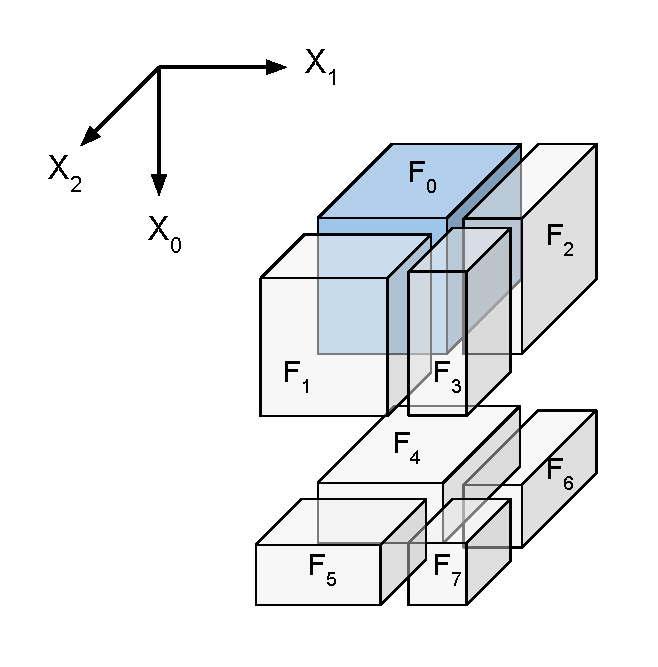
\includegraphics[width=0.5\textwidth]{./figures/figure_3.pdf}
  \caption{Division of a read block into write blocks. $F_0$, the write block represented in blue,
  is the output block containing the origin of the read block. $F_1$-$F_7$ are the intersections
  of the read block with the neighboring output blocks.
  Following this division, write blocks are merged using the scheme in Table~\ref{tab:fusion}.}
  \label{fig:nomenclature_overlaps}
  \end{figure}

\subsection{Peak memory}
To determine the peak memory used by a particular combination of read and
write blocks, one needs to determine the amount of data in the cache at
each iteration, which depends on how read and write blocks overlap. Since we were only able to find an analytical
upper bound of the peak memory usage, which in fact largely overestimates
it, we instead simulate each iteration of the \keep heuristic to measure
the cache size.

The simulation requires $\vert \texttt{readBlocks} \vert$ iterations. It
assumes that (1) read blocks are in the order used for array elements on
disk (C order in this paper), consistently with function \texttt{blocks}
and (2) write blocks are defined as described in the previous section.
Under these assumptions, we note that the
maximum number of sub-blocks of each type stored in the cache at any given
iteration is 1 for sub-blocks of type $F_1$, $A_2/R_2$ for sub-blocks of
type $F_2$ or $F_3$, and $A_1/R_1A_2/R_2$ for sub-blocks of type $F_4$ to
$F_7$. The simulation is therefore implemented with 3 circular buffers
$B_1$, $B_2$, $B_3$ of size 1, $A_2/R_2$ and $A_1/R_1A_2/R_2$ respectively.
At each iteration, the size of $F_1$ is added to $B_1$, the size of $F_2
\cup F_3$ is added to $B_2$, and the size of $F_4 \cup \ldots \cup F_7$ is
added to $B_3$. The sum of elements in $B_1$, $B_2$ and $B_3$ is computed
and its max across all iterations is returned as the peak memory
consumption.

\subsection{Number of generated seeks}
Similar to the
baseline, seeks generated by the \keep heuristic happen during reads (line
13 in Alg.~\ref{algo:generalrepartition}) and during writes (line 18).  To count the seeks generated
during reads, we note that the read process is dual to the write process:
writing in-memory blocks with end coordinates $\mathcal{M}$ to disk blocks
with end coordinates $\mathcal{D}$ generates the same number of seeks as
reading disk blocks with end coordinates $\mathcal{D}$ to in-memory blocks
with end coordinates $\mathcal{M}$.
We can determine this number using Equation~\ref{eq:seeks-baseline} without the last term:

\begin{eqnarray*}
  \textsc{seeks} \left(  \mathcal{M}, \mathcal{D} \right) &=&  A_0 A_1 c_2\left(\mathcal{M}_d, \mathcal{D}_d\right) + \\
                                                         &&  A_0 c_1\left(\mathcal{M}_d, \mathcal{D}_d\right) m_2\left(\mathcal{M}_d, \mathcal{D}_d\right) +\\
                                                         && c_0\left(\mathcal{M}_d, \mathcal{D}_d\right) m_1\left(\mathcal{M}_d, \mathcal{D}_d\right) + \\
                                                         && m_2\left(\mathcal{M}_d, \mathcal{D}_d \right) + \\
                                                         && (m_0+c_0)(m_1+c_1)(m_2+c_2)
\end{eqnarray*}
Function
\textsc{seeks} does not assume that $\mathcal{M}$ or $\mathcal{D}$ relate to
blocks of uniform shape. Therefore, it can be applied to the \keep
heuristics where write blocks are not necessarily of uniform shape.
The number of seeks generated by the \keep algorithm is given by:
\begin{equation}
  s_k = \textsc{seeks} \left(  \mathcal{R}, \mathcal{I} \right) + \textsc{seeks} \left( \mathcal{W}, \mathcal{O} \right)  \label{eq:seeks-keep}
\end{equation}

The first term represents the number of seeks required to read input
 blocks of end coordinates $\mathcal{I}$ into read blocks of end
 coordinates $\mathcal{R}$ whereas the second term represents the number of
 seeks required to write write blocks of end coordinates $\mathcal{W}$ into
 output blocks of end coordinates $\mathcal{O}$.

 The last two terms represent the number of input block openings and the number
 of output block openings, respectively.

 Function
 \texttt{generatedSeeks} is
 a direct implementation of Equation~\ref{eq:seeks-keep}.

\subsection{Implementation}

\tristan{mention tests; mention that we check seek model after each run; mention profiling}

\tristan{Mention array copies in Python, slicing doesnt copy data but references are copied
look at https://stackoverflow.com/questions/5131538/slicing-a-list-in-python-without-generating-a-copy}

We implemented the baseline and \keep heuristic in Python 3.7. The
project repository is available at
\url{https://github.com/big-data-lab-team/repartition_experiments}. It includes documentation on
how to install the package and its dependencies. The code used for the
experiments is also available in the same repository.
The implementation supports the HDF5 file format, but the code is modular
enough to accommodate other formats in the future.

To reduce the time requirements of brute-force search, we limit the testing
of candidate read shapes as follows in the implementation: starting from
$\hat r$ = ($\hat r_0$, $\hat r_1$, $\hat r_2$), we evaluate candidate read
shapes sorted by decreasing $X_1$ values, then by decreasing $X_0$ values.
We stop the search if the best number of seeks (\texttt{minSeeks} in
Alg.~\ref{algo:keep}) does not decrease for 10 iterations.

We could have passed the data from to read buffers to the cache by reference
which would have saved us the time of copying the data.
However, keeping a reference to the read buffers prevented them to be freed and
therefore increased the maximum amount of memory used drastically.
Therefore, we found that copying the data into the cache enabled us to stay below the
maximum memory consumption that we predicted at the buffer selection time.

%----------------------------------------
\section{Experiments}
%----------------------------------------
\label{sec:experiments}
\subsection{Seek model validation}

We tested our models against lighter implementations of the baseline and \keep
algorithms. We tested each model on 1,000 randomly generated cases.
To that aim, we first generate a random original array by multiplying 4 numbers
randomly drawn from ${2, 3, 5, 7}$, putting each number to the power 1 or 2
(again, randomly) and multiplying them:
$\hat r = (r,r,r)$ with $r = (x_0^{p_0}x_1^{p_1}x_2^{p_2}x_3^{p_3})$.
We then compute the divisors of $r$ and take two of them for the shapes of $I$
and $O$. We create 5 cases by picking 5 buffer shapes from the possible buffer
shapes given the configuration $(\hat r, I, O)$. We do the same after exchanging
$I$ with $O$. This gives us 10 configurations for a given randomly created $\hat r$.
We repeat the process until 1,000 cases have been randomly generated.
Then, for each case, we run our model to compute the number of seeks that the algorithm
should do, and compare it to the real number of seeks computed by running a light version
of the algorithm.

\begin{table*}
  \setlength{\tabcolsep}{2pt}
  \centering
  \caption{Input and output blocks shapes}
  \vspace*{-0.5cm}
   \begin{tabular}{c|ccc|ccc}
    \multicolumn{7}{c}{$A=(3500,3500,3500)$}\\
   \rowcolor{black!25}
          & \multicolumn{3}{c|}{\texttt{inBlocks}} & \multicolumn{3}{c}{\texttt{outBlocks}} \\
    \rowcolor{black!25}
  Config &      $I$      & $n_I$  & size &      $O$       & $n_O$  & size  \\
  \rowcolor{black!25}
     &               &        & (MiB)&                &        & (MiB) \\
   \hline
   0 & (875,875,875) & 64     & 1277    & (875,1750,875) & 32     &  2,555 \\
   1 &               &        &           & (700,875,700)  & 100    & 818 \\
   \rowcolor{black!10}
   2 & (350,350,350) &1,000   & 82        & (500,500,500)  & 343    & 238 \\
   \rowcolor{black!10}
   3 &               &        &           & (250,250,250)  & 2,744  & 29  \\
   4 & (175,175,175) &8,000   & 10        & (250,250,250)  & 2,744  & 29 \\
   \rowcolor{black!10}
   5 & (350,875,350) &400     & 204       & (500,875,500)  & 196    & 417 \\
   \rowcolor{black!10}
   6 &               &        &           & (350,500,350)  & 700    & 116 \\
   \end{tabular}
   \hfill
   \begin{tabular}{c|ccc|ccc}
    \multicolumn{7}{c}{}\\
    \multicolumn{7}{c}{$A=(8000,8000,8000)$}\\
   \rowcolor{black!25}
          & \multicolumn{3}{c|}{\texttt{inBlocks}} & \multicolumn{3}{c}{\texttt{outBlocks}} \\
    \rowcolor{black!25}
  Config &      $I$      & $n_I$  & size &      $O$       & $n_O$  & size  \\
  \rowcolor{black!25}
     &               &        & (MiB)&                &        & (MiB) \\
   \hline
   0 & (2000,2000,2000) & 64     & 15,258    & (2000,4000,2000) & 32     &  30,518 \\
   1 &               &        &           & (1600,1600,1600)  & 125    & 8,766 \\
   \rowcolor{black!10}
   2 & (800,800,800) & 1000     & 977    & (1000,1000,1000) & 512     &  1,907 \\
   \rowcolor{black!10}
   3 &               &        &           & (500,500,500)  & 4096    & 238 \\
   4 & (200,200,200) & 64000     & 15    & (250,250,250) & 32768     &  30 \\
   5 &               &        &           & (160,160,160)  & 125000    & 8 \\
   \rowcolor{black!10}
   6 & (400,400,400) & 8000     & 122    & (500,500,500) & 4096     &  238 \\
   \rowcolor{black!10}
   7 &               &        &           & (250,250,250)  & 32768    & 30 \\

   \end{tabular}
   \label{tab:exp}
\end{table*}
\subsection{Experiment conditions}
The experiments were run on a DELL-EMC PowerEdge C6420 server
with CentOS Linux release 8.1.1911 (Core), kernel release
$4.18.0-147.5.1.\textrm{el}8\_1.\textrm{x}86\_64$, 250GB of RAM,
6 $\times$ SSDs Intel SSDSC2KG480G8R (480~GB, xfs),
2 $\times$ Intel Xeon Gold 6130 CPUs @ 2.10GHz (16 cores/CPU, 2 threads/core).
The server was accessed through the SLURM batch manager.

We repartitioned two arrays of 2-byte elements (float 16): a "small" one (85.75~GiB)  of shape $A=(3500,3500,3500)$
and a "large" one (1024~GiB) of shape $A=(8000,8000,8000)$.
We used the input and output block shapes in Table~\ref{tab:exp}.
We repartitioned the small array with $m$=275~GiB (256~GB), 8.6~GiB (8~GB)
 and 4.3~GiB (4~GB), to benchmark the baseline and \keep algorithms with different
 memory constraints. For the large array we used $m$=256~GB only.
The memory was controlled through SLURM's cgroup-based memory requirement,
which means that $m$ was the total amount of RAM allocated to the
repartitioning task, including anonymous memory and cache. Swapping was
disabled.

A single disk was used when processing the small array. However, for the
large array, the 6 disks available on the server were used as the capacity of a single disk was not
enough to accommodate the input or the output blocks. We used the disks in
round-robin.

We did 5 repetitions of each configuration for the small array, and 1
repetition for the large array. The page cache was flushed at the beginning
of each repetition.


\subsection{Results}

\begin{figure*}
  \centering
  \begin{subfigure}{\textwidth}
    \caption{Number of seeks (log scale)}
    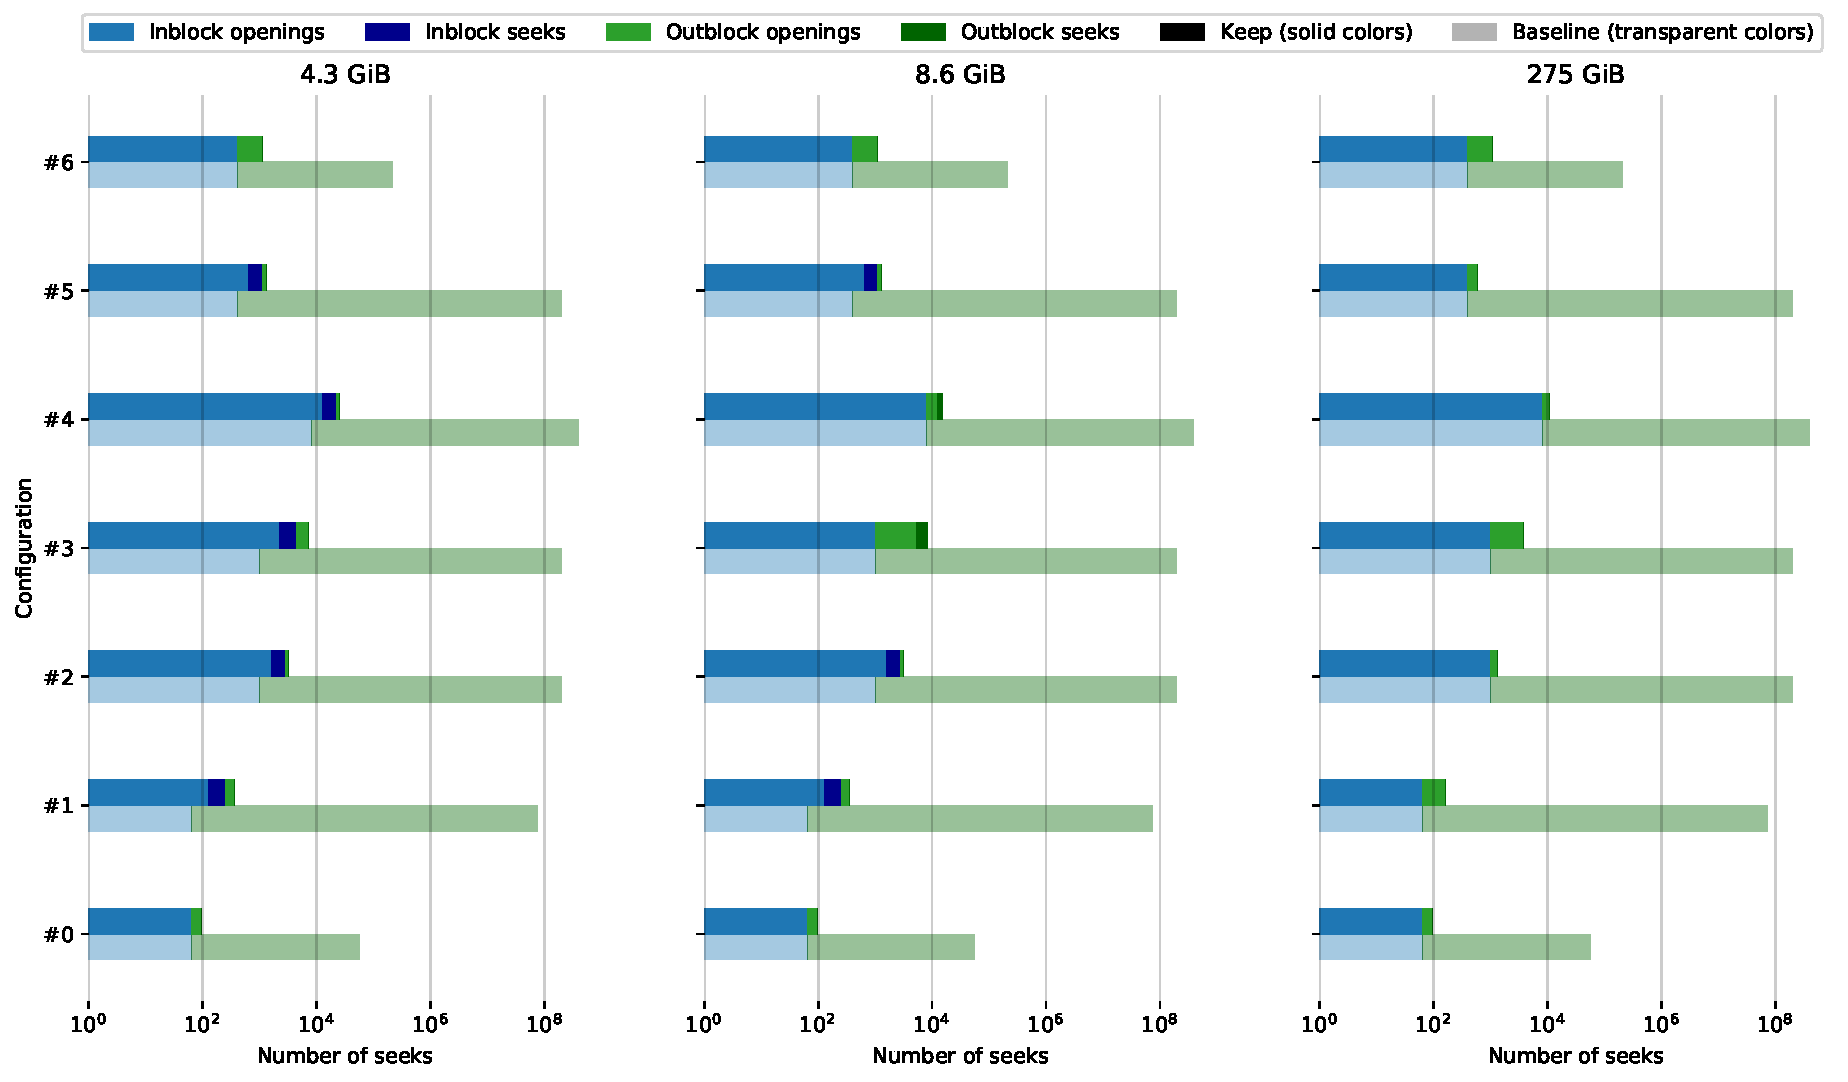
\includegraphics[width=\textwidth]{./figures/seeks_3500.pdf}
    \label{fig:seeks_3500}
  \end{subfigure}
  \begin{subfigure}{\textwidth}
    \caption{Processing time}
   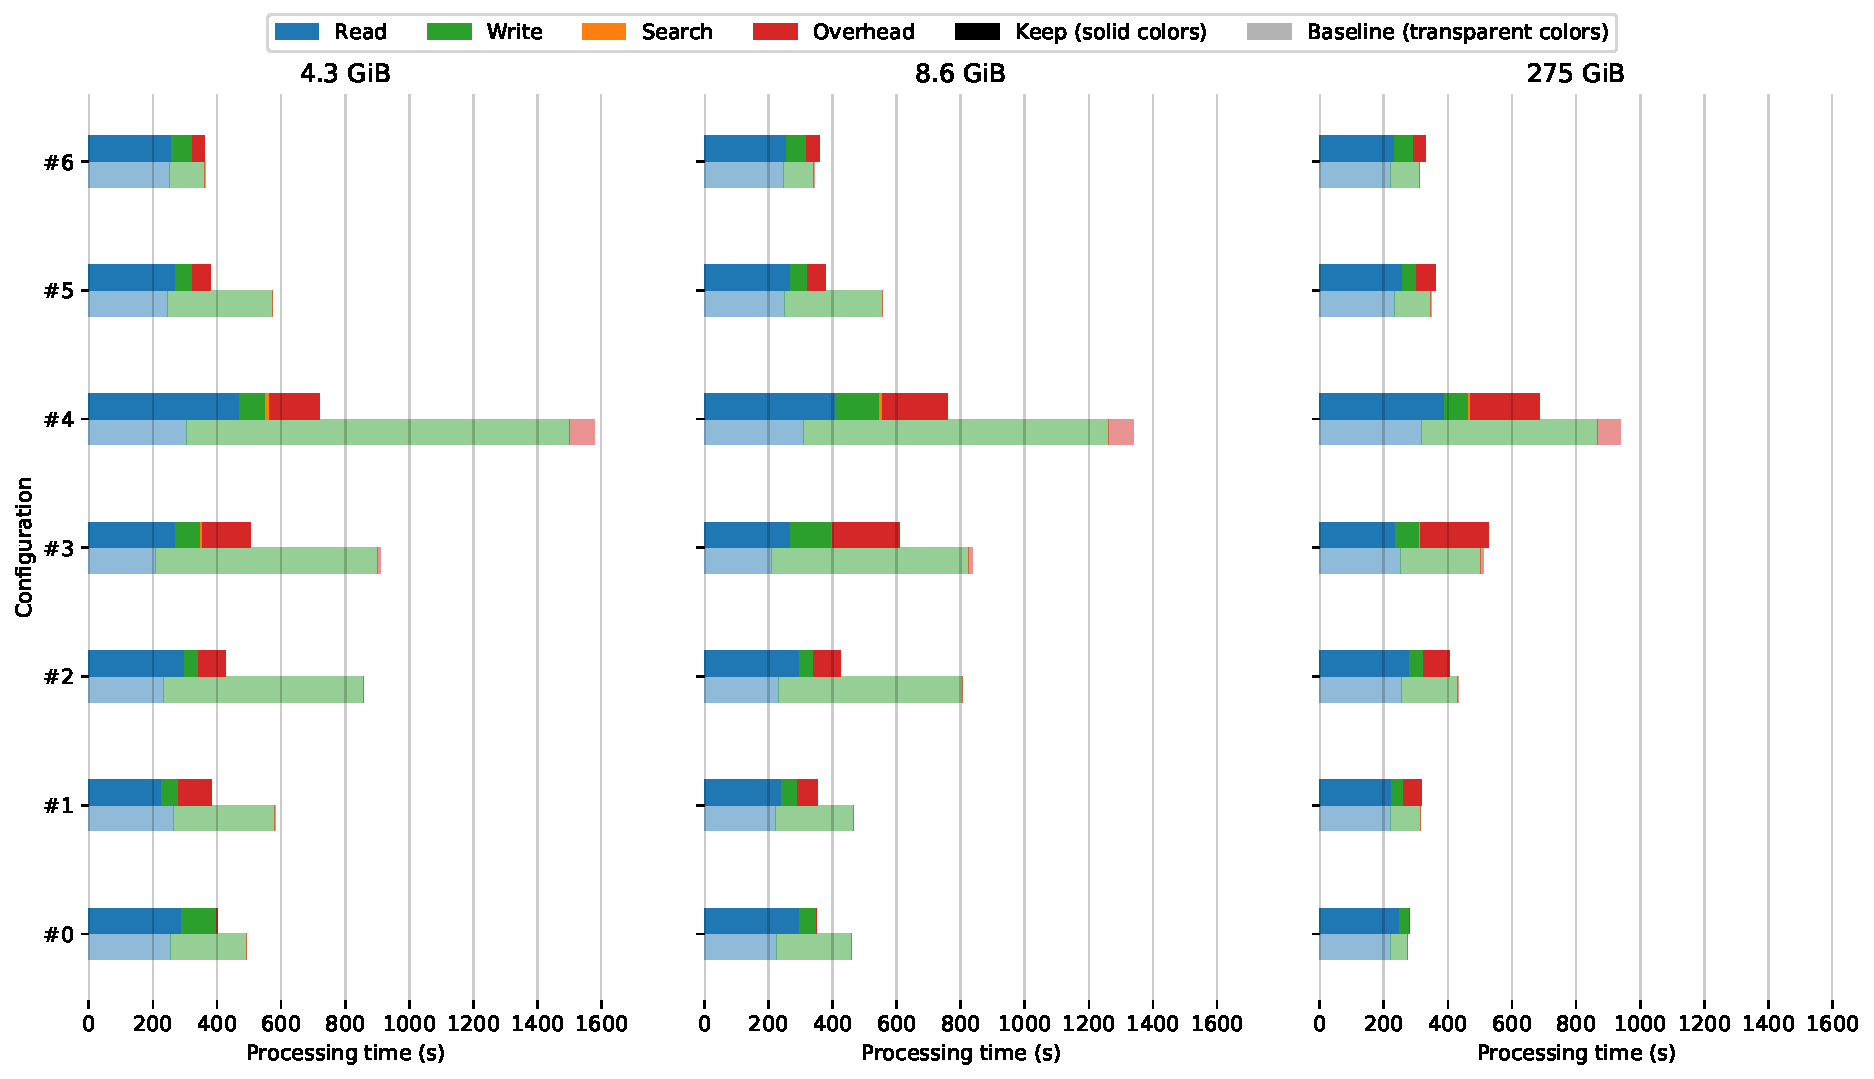
\includegraphics[width=\textwidth]{./figures/time_3500.pdf}
  \label{fig:time_3500}
  \end{subfigure}
  \caption{Repartitioning results for the small array (85.75~GiB). Averages on 5 repetitions. \textbf{(a)} Compared to baseline, the \keep heuristic
  reduces the number of seeks by four orders of magnitude. \textbf{(b)} The \keep heuristic provides speed-up factors of up to 2.5 (configuration 4).}
  \label{fig:3500}
\end{figure*}


\subsubsection{Small array (85.75~GiB)}

Results are shown in Figure~\ref{fig:3500}.
By design, the number of seeks is drastically reduced by the \keep
heuristic compared to baseline (Fig.~\ref{fig:seeks_3500}), by a factor of
90,000 on average. In configurations 1 to 5 in particular, baseline
requires up to $10^8$ seeks while the \keep heuristic only requires up to
$10^4$.

This reduced seeking translates to important reductions of the
repartitioning time (Fig.~\ref{fig:time_3500}). Compared to baseline, the
\keep heuristic provides speed up factors of up to 1.4 for
$m$=275~GiB, 1.9 for $m$=8.6~GiB, and 2.2 for $m$=4.3~GiB.
Speed-up is only observed when baseline requires O($10^8$) seeks, which occurs
in configurations 1 to 5: lower amounts of seeks don't seem to have an effect on
I/O time. Speed-up is mostly coming from write time reduction, since
baseline read complete input blocks without seeking.


% Considering run 4 which shows the most important differences in terms of
% processing time, the amount of seeks have been reduced from about 100 millions
% seeks to thousands of seeks.
% We also remark that although the number of seeks have been reduced from millions
% to thousands of seeks for runs 1 to 5, the reduction in processing time does not
% follow linearly the reduction in the number of seeks.
% This is probably due to the fact that some seeks are more costly than others,
% which has not been taken into account in our problem formulation.

The baseline performances improve drastically with the amount of memory
allocated to the repartitioning. For $m$=275~GiB, repartitioning times of
baseline and \keep are on par for all configurations except configuration
4. This is most likely due to the use of asynchronous write back to disk
through the Linux page cache. In our experiments, the ratio of "dirty"
data, the cache data waiting to be written to disk, was set to 40\%, a
common value for compute nodes, which means that the small array entirely
fit in memory for $m$=275~GiB. The \keep strategy is mostly useful for
arrays that do not fit in page cache memory.

The overhead of the \keep heuristic consists of search time
(Alg.~\ref{algo:keep}) and cache management (data copy to/from cache in
Alg.~\ref{algo:generalrepartition}). While search time is negligible, cache
management is substantial except for configuration 0 where the total number
of blocks is limited.


Table~\ref{tab:buffer_shapes} shows the read block shapes selected by the
\keep heuristic. The optimal shape $\hat r$ was used for all configurations with $m=$ 275~GiB.
  \begin{table}
    \centering
    \caption{Read block shapes and peak memory estimates selected by the
    \keep heuristic to repartition the small image.}
     \begin{tabular}[t]{cccc}
     \hline
     \rowcolor{black!25}
    Config &      $m$=4.3 GiB   & $m$=8.6 GiB     & $m$=275 GiB  \\
    0      &   (875, 1750, 875)* & (875, 1750, 875)* & (875, 1750, 875)* \\
           &    2.8 GiB         & 2.8  GiB        & 2.8  GiB             \\
           \rowcolor{black!10}
    1      &   (700, 875, 875)  & (700, 875, 875) & (875, 875, 875)* \\
           \rowcolor{black!10}
           &    1.8  GiB        & 1.8  GiB        & 15.3  GiB              \\
    2      &   (500, 700, 700)  & (500, 700, 700) & (700, 700, 700)* \\
           &    2.1  GiB        & 2.1  GiB        & 12.2  GiB             \\
           \rowcolor{black!10}
    3      &   (250, 350, 350)  & (350, 350, 350) & (350, 350, 350)* \\
           \rowcolor{black!10}
           &    0.45 GiB        & 5.5   GiB       & 5.5   GiB            \\
    4      &   (250, 350, 350)  & (350, 350, 350)* & (350, 350, 350)*  \\
           &    0.45 GiB        & 5.5  GiB        & 5.5   GiB            \\
           \rowcolor{black!10}
    5      &   (500, 875, 700)  & (500, 875, 700) & (700, 875, 700)* \\
           \rowcolor{black!10}
           &    1.0  GiB        & 1.0  GiB        & 11.5  GiB             \\
    6      &   (350, 875, 350)*  & (350, 875, 350)* & (350, 875, 350)* \\
           &    1.2  GiB        & 1.2  GiB        & 1.2   GiB            \\
     \hline
     \end{tabular}
     * selected read block shape was $\hat r$
     \label{tab:buffer_shapes}
  \end{table}

\subsubsection{Large array}

\tristan{We can't really present these results unless the overheads are fixed,
including cache management and read times.}

Given the 250~GB RAM available, the read buffer shapes tested were always equal to
the input aggregates' shapes.
Globally, one can see on Figure~\ref{fig:time_8000} that apart from run 2 the \keep
strategy and baseline are pretty equivalent, and for 5 runs over 8 the \keep
strategy is slightly faster.
There is no important improvement, however, which is mainly due to 3 bottlenecks:
\begin{itemize}
  \item the overhead time
  \item the preprocessing time
  \item the read time
\end{itemize}

It seems logical to get an overhead time that explodes, especially in run 2, as
it was already important on the small array. As it is mostly due to cache manipulations,
a bigger array implies bigger data transferred during these cache manipulations.

Interestingly, the preprocessing time can be very large.
The preprocessing time includes the computation of the write buffers and the
computation of a Python dictionary associating each buffer with the output blocks
it intersects. The latter operation can be very expensive when there are a lot
of buffers.

The experiment on a big array was worth it as it clearly shows a limit
of the \keep strategy: We can see on Figure~\ref{fig:time_8000} that for runs
2 to 4, the write time (in green) has been tremendously reduced, but at the
cost of an increase in read time.

Finally, one can see on Figure~\ref{fig:seeks_8000} that in this experiment, too,
the \keep strategy succeeded in reducing the number of seeks significantly. Once
again, the reduction in processing time is also non-linear with the reduction in
seeking.

\begin{figure*}[h]
  \centering
  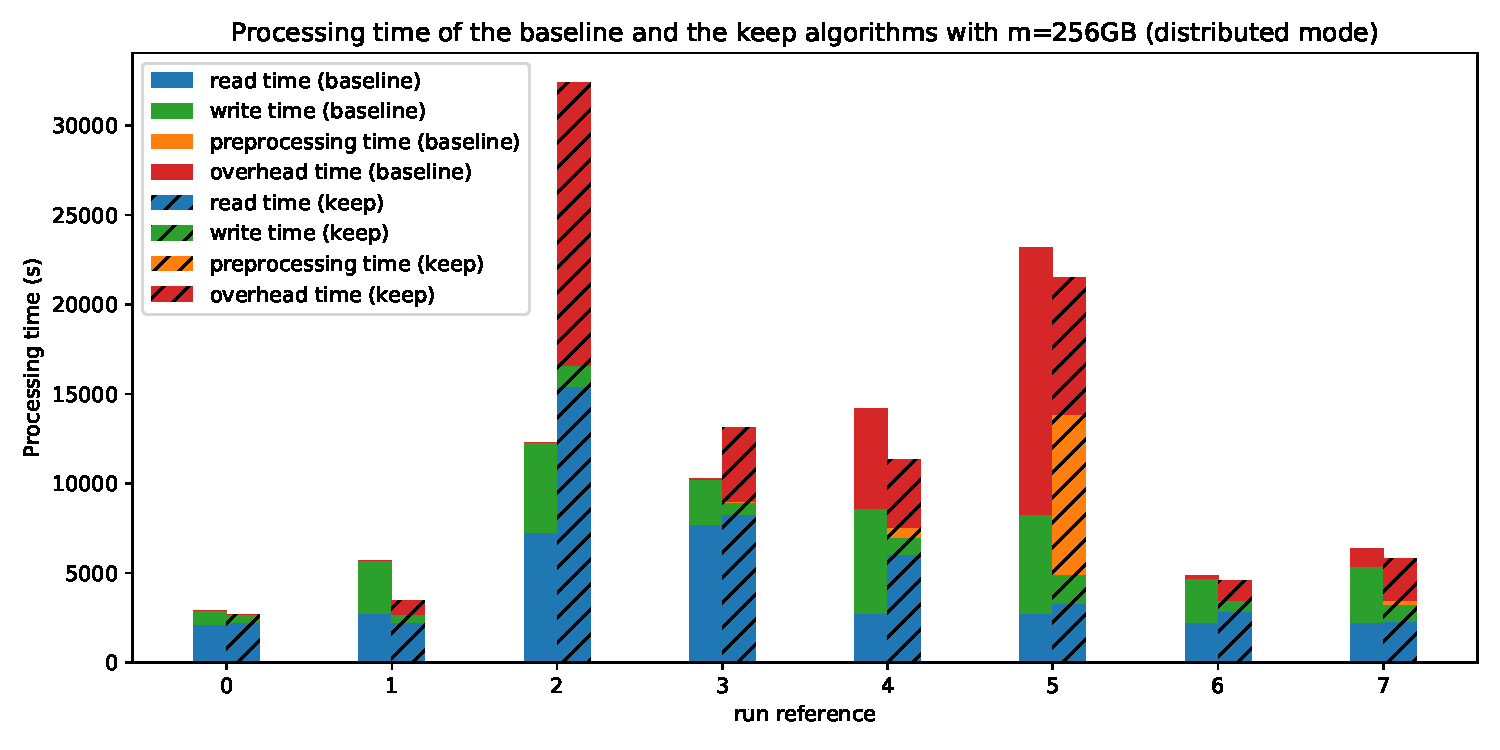
\includegraphics[scale=0.36]{./figures/time_8000.pdf}
  \caption{Results in terms of processing time for the keep and baseline algorithms. From left to right, the results are presented for 256, 8 and 4GB of available main memory.}
  \label{fig:time_8000}
\end{figure*}

\begin{figure*}[h]
    \centering
    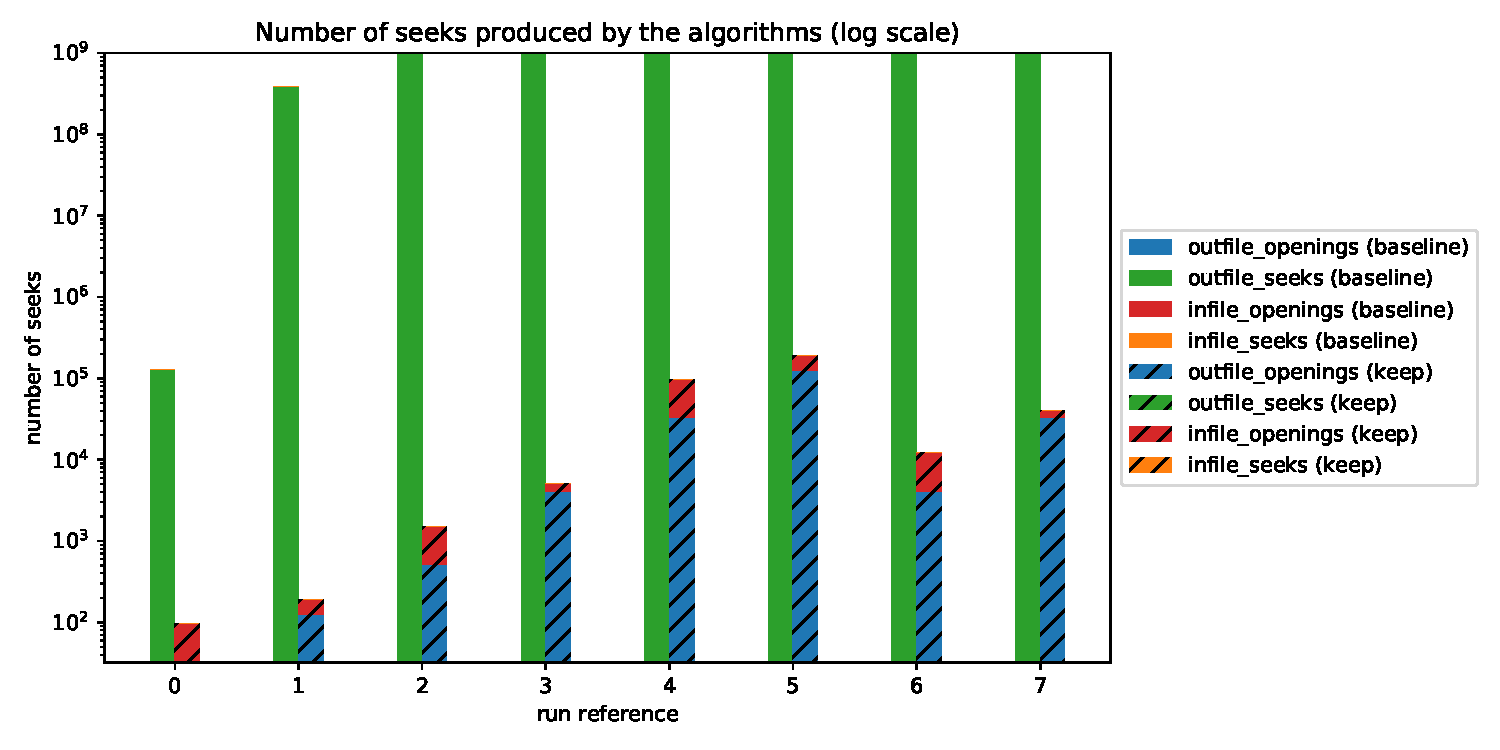
\includegraphics[scale=0.36]{./figures/seeks_8000.pdf}
    \caption{Results in terms of seeks for the keep and baseline algorithms. From left to right, the results are presented for 256, 8 and 4GB of available main memory.}
    \label{fig:seeks_8000}
\end{figure*}

%----------------------------------------
\section{Discussion}
%----------------------------------------
\tristan{Tristan to refocus the discussion and conclusion}

%
The \keep heuristic can reduce the number of seeks required to repartition an array
from millions to thousands compared to the baseline
algorithm. As a result, write time is drastically reduced and speed-up
factors of up to \mytodo{x} are observed. Speed-up factors are expected to
increase with the size of the repartitioned array; in 3D, speed-up is
proportional to $A_0$$A_1$ when enough memory is available to avoid cuts in
dimension 2. Speed-up factors are also expected to increase with the dimension of
the repartitioned array; in dimension $d$, speed-up is proportional
to the product of the first d-1 $A_i$ when enough memory is available.
Therefore, the \keep heuristic is adapted to the repartitioning of large
multi-dimensional arrays in the current context of growing data volumes.

\subsection{Relevant extensions}

% Memory
Allocating only reasonable amounts of working memory, 4.3~GiB for an array
of 85.75~GiB in our experiments, seems to be sufficient to remove most of
the seeks required for the repartitioning. This is consistent with the fact
that the \keep heuristic only stores partial output blocks in cache, until
they can be combined into complete output blocks. In the future, it would
be interesting to derive an upper bound of the peak memory consumption, to
generalize this observation beyond the particular input and output block shapes
tested in our experiments.

% Page cache
The memory page cache provided by the Linux kernel plays a significant role
in the repartitioning problem when the amount of memory increases. When
repartitioning a 85.75~GiB array with 275~GiB of working memory, all the
output blocks are written to memory and asynchronously flushed to disk,
bringing the baseline algorithm on par with the \keep heuristic. This is
not surprising given the importance of page cache for I/O intensive
applications~\cite{hayot2019performance}. The Linux kernel provides other
relevant I/O strategies such as readahead and clustered writes that may
interfere with the \keep heuristic. Incorporating awareness of kernel I/O
strategies into the repartitioning algorithm may further enhance
performance.

% Parallelization and clusters
Most applications would process large multi-dimensional arrays in parallel,
on a multi-core computer or on an HPC cluster. The \keep heuristic is
directly applicable to multi-core environments, assuming sequential I/Os.
The case of HPC clusters, however, it would have to be extended to consider network data
transfers. In addition, HPC clusters would most
likely store input blocks on a parallel file system such as Lustre where
files are striped across multiple disks and nodes. An extended formulation of the
repartitioning problem would be required in this context.
It would be interesting to integrate such an extension in the Dask engine,
a popular parallelization framework of the SciPy ecosystem~\cite{matthew_rocklin-proc-scipy-2015}.
In particular, the \keep heuristic would interface nicely with the \texttt{dask.array} API.

\tristan{Timothée, you wrote this: "there is still margin for improvement in optimizing
the read time.". Could you explain why?}
\timothee{ce que je veux dire c'est qu'au final la méthode de "buffer extension" permet de réduire les seeks en écriture mais pas en lecture alors que de base on souhaitait que ça réduise en écriture ET en lecture}

Other array manipulation problems could benefit from a similar approach.

% Buffer ordering

% Seek types

% The buffer order is important when using the keep strategy, as it defines when
% a piece of data will be loaded and when a write buffer will be complete, hence
% ready to be written down and freed from the cache.
% Representing the read buffers by a complete bidirectional graph in which each
% vertex is a buffer, we can model the problem as kind of a complex shortest path
% problem.
% Indeed, for a given buffer shape $B$, we want to find the read buffers order
% that will keep the amount of memory used by the re-partition algorithm low.
% Solving this problem would incur more infering at runtime and a potentially
% complex algorithm to run.
% We decided to keep things simple using a naive buffer order, as the goal of
% this study was primarily to assess if the keep algorithm works.

% Using the keep strategy, one may order the buffer loadings to reduce the maximum
% quantity of extra data stored in memory, hence, reducing the amount of seeks.
% For example, if the shape mismatches occur only in the $k$ axis, loading the
% buffers in this direction will enable recycling the extra data in cache,
% resulting in a smallest memory consumption over time.
% The memory saved thanks to a smart
% ordering could enable the storage of more extra data in memory using the
% keep strategy, further reducing the amount of seeks produced.

% As explained in the discussion, the buffer ordering problem is complex and does
% not seem easily solvable.
% This study uses a naive order which is, again, the inverse storage order.
% The reason for that order is that as it is more important to keep data in the
% $k$ dimension to save seeks and we assume that $B_k=\hat r_k$, it seems
% reasonable to load the buffers in the $k$ dimension first.
% Note that using such
% an order recycles extra data in the $k$ dimension first; It is therefore
% more efficient when the biggest shape mismatch between the input and output
% blocks is in $k$.

% Thankfully, the impact of the buffer ordering on performance can be
% mitigated. Indeed, the impact of the buffer ordering depends on the size of the
% mismatches. One can reduce the amount of extra data by using smallest blocks: Even
% if the overlap between the input and output files is big with respect to their
% size, the area/volume of the overlap will be kept small.

% Finally, it could be interesting to try identifying the type of seeks that are
% more costly than the others and focus future implementations of the re-partition
% algorithm to reduce such costly seeks.


% Split and merge
% \subsection{Split and merge}

% Special cases of the re-partitioning problem occur when $I=A$ (``split''
% problem) or when $O=A$ (``merge'' problem). Two strategies were introduced
% in~\cite{seqalgorithms} to address these problems: the ``multiple" and the
% ``clustered" strategies. In these strategies, every read block is directly
% written to the destination output files, that is, \texttt{readBlocks} and
% \texttt{writeBlocks} are identical ($R=W$). The only difference between the
% multiple and the clustered strategies lies in the selection of $R$.

% In the split problem, the naive strategy defines the read blocks as having
% the same shape as the output blocks ($R$=$O$). The read blocks are
% iteratively loaded from $A$ and entirely written to the appropriate output
% block. The clustered strategy, however, loads as many contiguous read
% blocks of shape $O$ as possible to fit in $m$. $R$ is therefore a multiple
% of $O$. Depending on the amount of main memory available, read blocks may
% be loaded individually, by entire block columns, or by entire block slabs.
% Although this strategy allows to write each output block in one seek, the
% clustered strategy is limited by the fact that it does not optimize the
% reading step. In the general re-partitioning problem, one can expect the
% clustered strategy to perform poorly as it reads an output block regardless
% of its spread among input blocks.

% The multiple strategy
% aims at not doing any seek while reading \textit{and} writing:
% both the input and the output blocks are read/written contiguously. In
% terms of Algorithm~\ref{algo:generalrepartition}, it means defining read blocks as
% contiguous parts of the input array and write blocks as contiguous parts of
% the output arrays. Although the multiple strategy does not seek while reading or writing, it
% requires many switches between output blocks.

% As stated in the introduction, the split and merge tasks are special cases of
% the repartition task. This observation leads us to think that maybe one could find
% one optimal algorithm for the split, merge and repartition tasks.

% If we were to use the keep algorithm with $I=R$, we would read the input data
% in slices, exactly like the multiple strategy. The only difference between the
% two strategies, however, is that if some remainders appear at the bottom of the
% buffer, the keep algorithm would keep it to try to read and write files in one
% seek. Not only the keep algorithm tries to limit seeking into the files but it
% also tries to limit switching between the files. It would be interesting to
% compare the two algorithms for the split/merge tasks to see if the keep
% implementation brings similar results or any kind of improvement.

% ROIs
\subsection{ROI extraction}
The Region Of Interest (ROI) extraction problem is a related problem that still
needs to be addressed.
A solution using chunking as been introduced in~\cite{optimal_chuking}.
The authors define an array partitioned into chunks of equal shapes and then
define a query as an arbitrary subarray of the input, chunked, array.
They define the optimal chunking problem as finding the optimal chunk such
that the expected number of chunks retrieved to answer the query is minimal.

In our opinion, the solution in~\cite{optimal_chuking} is limited due to the
need of historical or theoretical workload and the necessity to repartition the
input array into an ``optimal" chunk shape.
We would prefer letting the application choose the appropriate chunk shape
regarding its needs and not needing to estimate the processing workload.
We define the ROI extraction problem as follows: Finding an algorithm that takes
as input an arbitrary chunk shape and extracts the ROI data from the chunks with
the less number of seeks as possible.



% Although the keep algorithm can be 2 times faster than the baseline algorithm
% in some cases, our implementation suffers from a tradeoff between optimizing
% the processing time and predicting the maximum amount of memory consumed.
% In some non-complex cases, the baseline algorithm can be as efficient as the
% keep algorithm.
% Moreover, the baseline algorithm seems to take advantage of the surplus of
% main memory available in the node, although in theory it is supposed to use
% only the size of one input block in bytes at a time.
% This does not seem to be the case of the keep algorithm for which the maximum
% amount of main memory consumed can be estimated before run.

%----------------------------------------
\section{Conclusion}
%----------------------------------------

Multidimensional array chunking is a routine for scientists nowadays.
That is why efficiently processing such arrays is of major importance in the big data era.

Splitting and merging arrays has been successfully done, we therefore attempted
to solve the next step: the re-partitioning problem.
This problem consists of efficiently re-writing a chunked array to change the shape of the blocks.
We think that solving this problem could enable us to solve the ROI (region of interest)
extraction problem in the future, which is also a very common problem for scientists.
We formally defined the re-partitioning problem together with a \emph{baseline algorithm} to solve it.
We also presented the \emph{keep algorithm} to reduce the number of seeks produced during
the re-partitioning and hopefully reduce the processing time of such task.
The keep algorithm reduces the number of seeks by
(1) constraining the read buffers shape to minimize the read time, and
(2) leveraging a ``cache" to minimize the write time.

Although the re-partitioning problem is more complex than splitting/merging chunks,
we proved that it can be optimized and that it is possible to reduce the
processing time significantly.
Surprisingly, however, the baseline algorithm has been found to perform pretty
well when there is a lot of memory available as it leverages the page cache to
speedup computations without reducing the number of seeks.
For now, the keep algorithm may be more interesting than the baseline algorithm
only when the memory constraint is important ($m$ small compared to the array size).

In the future, the algorithm performances may be improved by finding a variant
to the keep algorithm that also reduce the read time significantly,
identifying and focusing on reducing the most expensive seeks,
and finally, finding parallel and/or distributive versions of the keep algorithm.

%----------------------------------------
\section{Acknowledgments}
%----------------------------------------

The computing platform was obtained with funding from the Canada Foundation for Innovation.

\bibliography{Bibliography}
\bibliographystyle{ieeetr}

\end{document}
